\begin{frame}{SaM Solutions}
  \begin{center}
    
\includegraphics{sam-solutions-elinux}
  \end{center}
\end{frame}

\begin{frame}{SaM Solutions. Начало истории}
  \begin{block}{Август 2011}
    Принято решение о развитии направления Linux \& Embedded
  \end{block} \pause

  \begin{block}{Сентябрь-ноябрь 2011}
    Подготовка бизнес-плана:
    \begin{itemize}
      \item организация взаимодействия с FOSS-community
      \item оплата выезда сотрудников на профильные конференции\footnote{с последующим принудительным обменом информацией внутри компании: knowledge sharing session}
      \item профессиональное обучение и переподготовка
    \end{itemize}
  \end{block} \pause

  \begin{block}{Январь 2012}
    бизнес-план утверждён и начал выполнятся
  \end{block}

\end{frame}

\begin{frame}{SaM Solutions. Постановка вопроса}
  \alert{Проблема}:
  \begin{itemize}
    \item Проекты есть, людей нет
    \item Те, кого нанимаем - не тянут и уходят
    \item Люди не знают инструментальную среду Linux
    \item Корочки курсов QA не дают нам ничего 
  \end{itemize} \pause

  \alert{Тенденции}:
  \begin{itemize}
    \item Сегмент Linux стремительно растёт
    \item Специалистов никто не готовит 
    \item Специалисты уезжают
  \end{itemize} \pause
    
\end{frame}

\begin{frame}[fragile]{Доступно о кадрах}
 
  \begin{center}
    \Large \alert{Количество и качество \newline специалистов к объёму работы \newline стремительно падает} 
  \end{center}
  \begin{tabular}{l r}
    
\includegraphics[height=5cm]{popa} &
    
\includegraphics[height=5cm]{penguin} \\
  \end{tabular}

\end{frame}

\begin{frame}{SaM Solutions. Стажировка Linux QA}
  \alert{Решение - чучхэ, опора на свои силы}

  \begin{itemize}
    \item Свои преподаватели
    \item Программа, адаптированная к своим проектам
    \item Свой учебный класс
    \item Отбор из хорошо мотивированных соискателей\footnote{любого возраста и рода занятий}
  \end{itemize} \pause


  \alert{Набор}
  \begin{itemize}
    \item конкурс 3 человека на место
    \item 10 человек отобрано
    \item занятия с 4 января по 15 февраля
    \item 3 раза в неделю по 3 часа
  \end{itemize}

\end{frame}

\begin{frame}{Организация курса. Блоки}
  
  \begin{itemize}
    \item Независимые блоки с практическим и теоретическим материалом по выбранной теме.
    \item Примеры блоков: Shell, Управление процессами, Файловая система Unix, Обработка текста.
    \item Каждый блок - от 0.5 до 3 занятий.
    \item Блоки сразу создаются для повторного использования.  \newline
      Могут быть прочитаны как отдельные разовые курсы повышения квалификации.
  \end{itemize}

\end{frame}

\begin{frame}{Ранняя публикация результатов}

  \Large
  \begin{center}
    \alert{Release early, release offen} 

    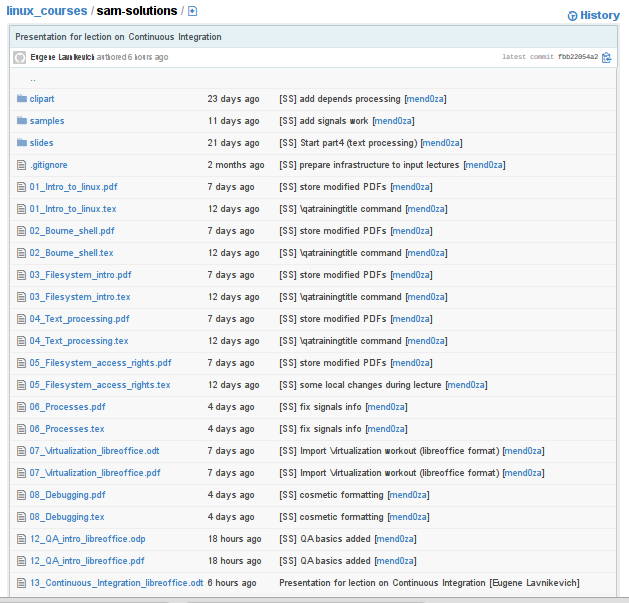
\includegraphics[height=5cm]{github}

    \alert{Go github!}
  \end{center}
  
\end{frame}

\begin{frame}{Результат}
  \begin{center}
    \large 
    Формально:
    \begin{itemize}
      \item список рекомендованных к найму 
      \item понедельник, 18 февраля - вручение дипломов  
      \item плюс 10 человек в экосистеме линукс
    \end{itemize} \pause

    Неформально:
    \begin{itemize}
      \item мотивированные обученные люди 
      \item невысокие ЗП на старте
      \item высокая лояльность к компании
    \end{itemize}
  \end{center}
\end{frame}
